\begin{figure}[!]
    \begin{subfigure}{\textwidth}
    \centering
    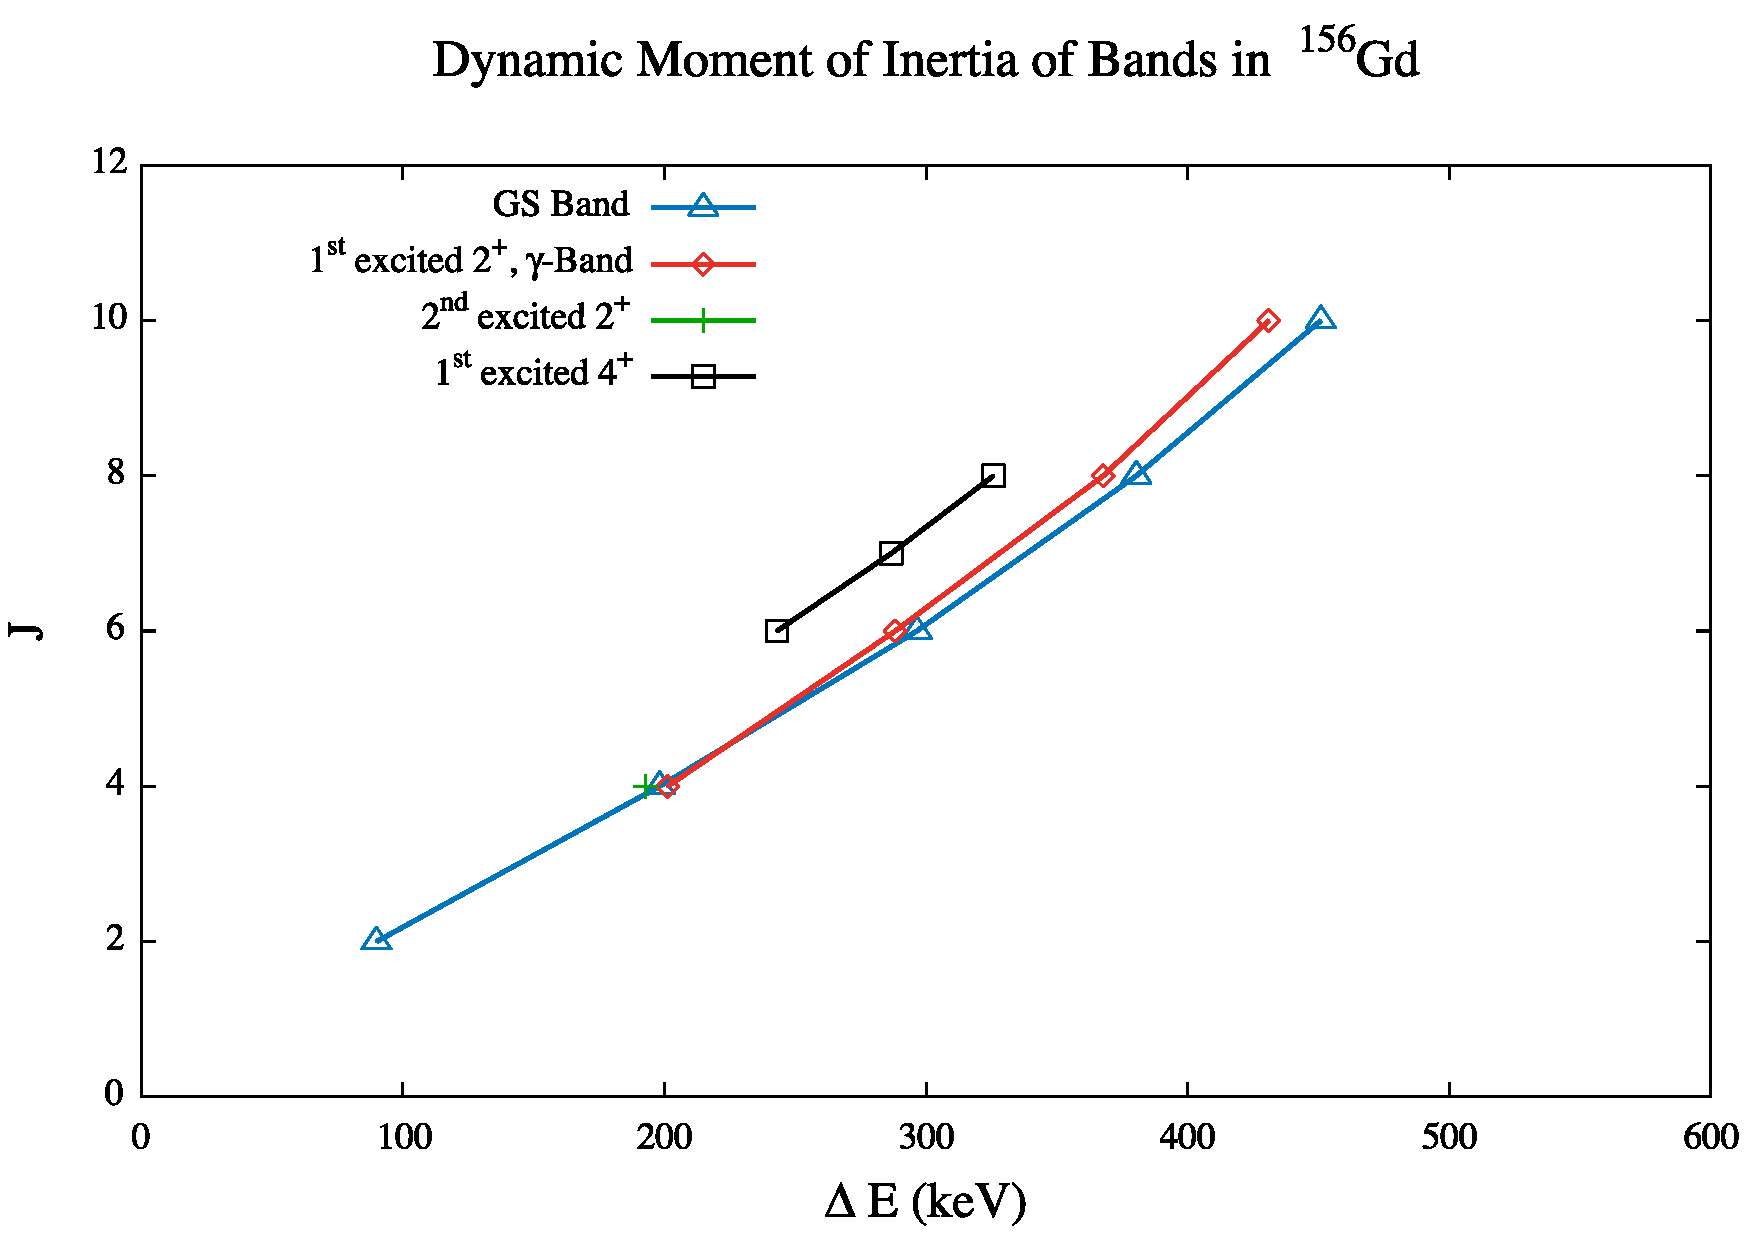
\includegraphics[scale=0.4]{Discussion/156_Dynamic.pdf}
    \caption*{(a)}
    \end{subfigure}
    \begin{subfigure}{\textwidth}
    \centering
    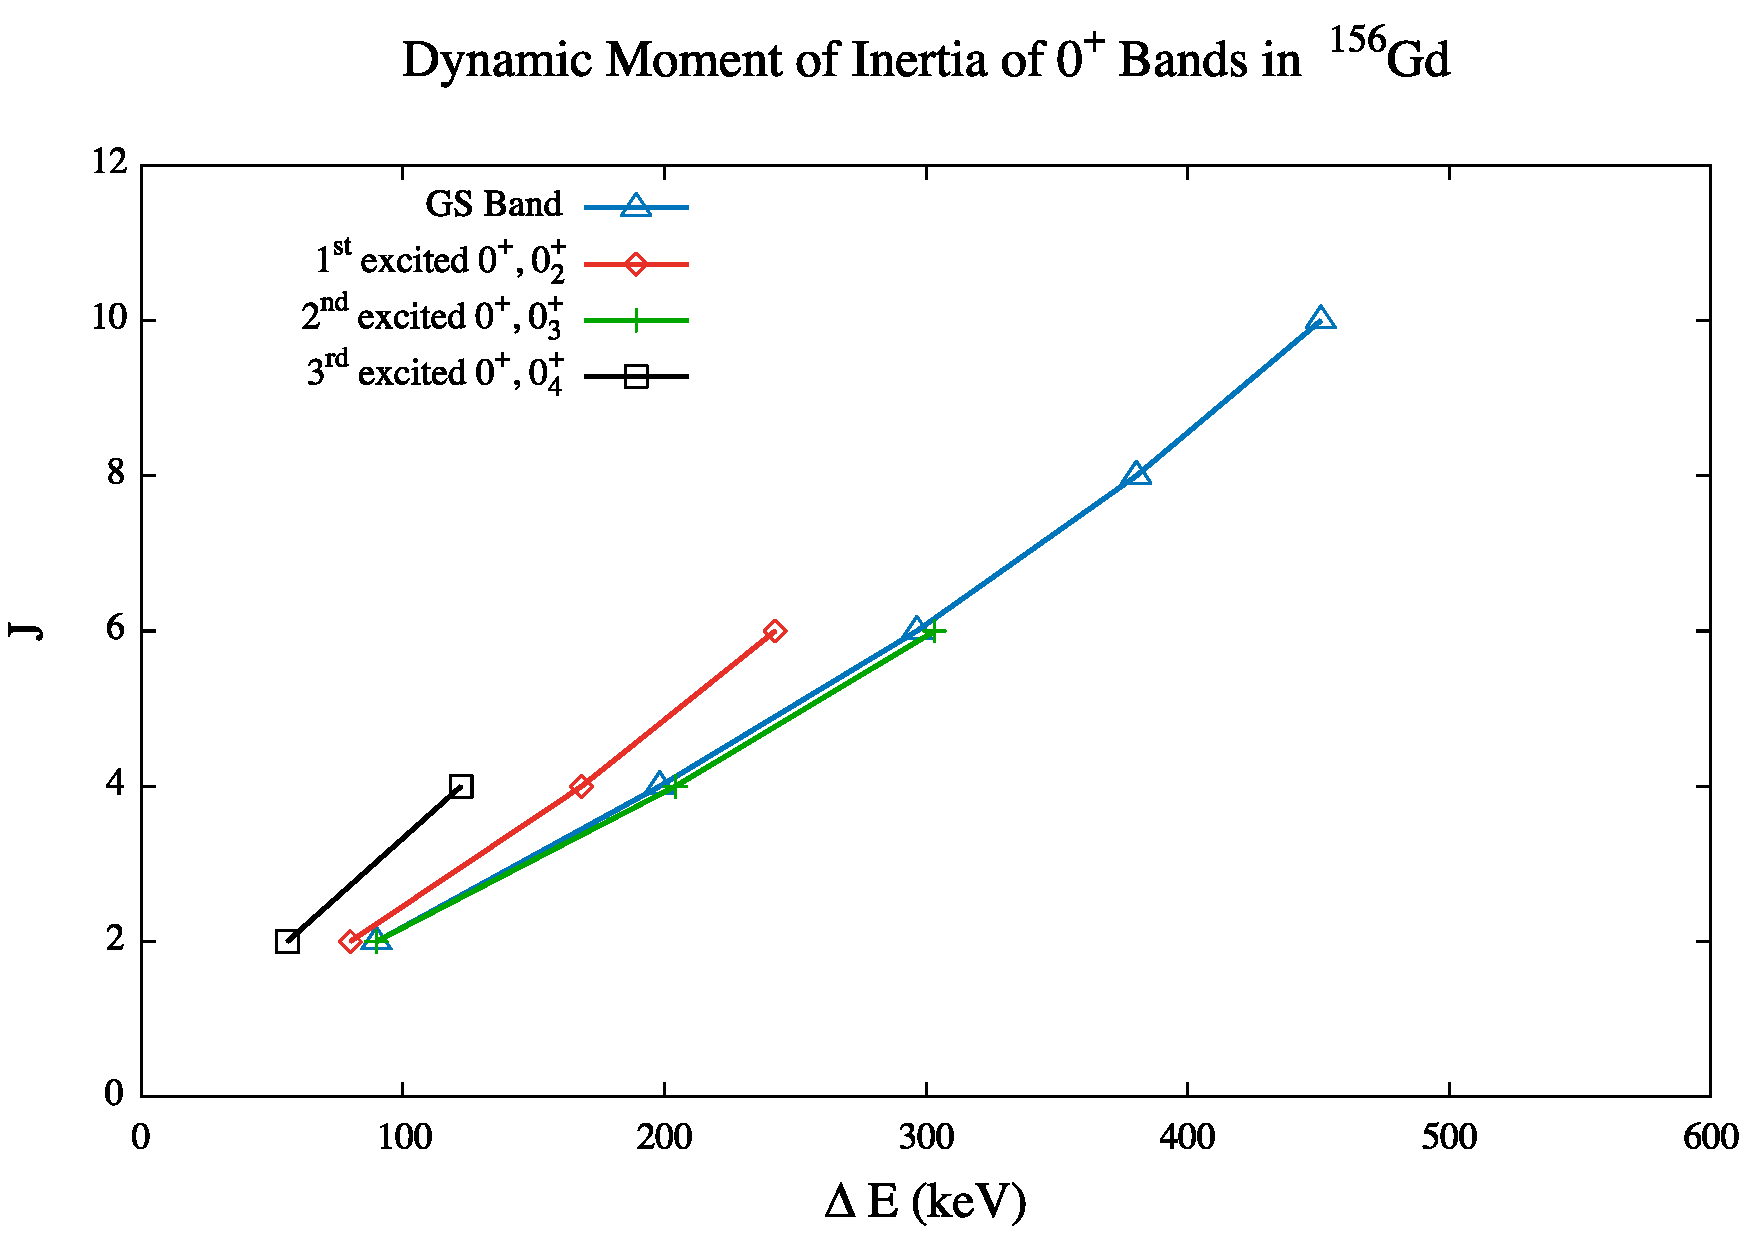
\includegraphics[scale=0.4]{Discussion/156_Dynamic0.pdf}
    \caption*{(b)}
    \end{subfigure}
    \caption{(a) The dynamic moments of inertia of the non-$0^+$ bands seen in the experiment. As is seen visually and with the slopes, the ground state band and the $\gamma$ band have similar moments of inertia, and overlap within two standard deviations. (b) The dynamic moments of inertia of the four $0^+$ bands seen in the experiment. As is seen visually and with the slopes, the ground state band and the first excited $0^+$ band have very similar moments of inertia.}
    \label{fig:156_Dynamic}
\end{figure}